\documentclass{article}

% if you need to pass options to natbib, use, e.g.:
%     \PassOptionsToPackage{numbers, compress}{natbib}
% before loading neurips_2023

\usepackage[preprint]{neurips_2023}


% to compile a preprint version, e.g., for submission to arXiv, add add the
% [preprint] option:
%     \usepackage[preprint]{neurips_2023}
% to compile a camera-ready version, add the [final] option, e.g.:
%     \usepackage[final]{neurips_2023}
% to avoid loading the natbib package, add option nonatbib:
%    \usepackage[nonatbib]{neurips_2023}
\usepackage[utf8]{inputenc} % allow utf-8 input
\usepackage[T1]{fontenc}    % use 8-bit T1 fonts
\usepackage{hyperref}       % hyperlinks
\usepackage{url}            % simple URL typesetting
\usepackage{booktabs}       % professional-quality tables
\usepackage{amsfonts}       % blackboard math symbols
\usepackage{nicefrac}       % compact symbols for 1/2, etc.
\usepackage{microtype}      % microtypography
\usepackage{xcolor}         % colors
\usepackage{svg}

\usepackage[caption=false]{subfig}
\usepackage[font=small,skip=3pt]{caption}

\usepackage{algorithm}
\usepackage{algpseudocode}
\usepackage{amsmath}
\usepackage{amssymb}
\usepackage{todonotes}
\usepackage{enumitem}

\renewcommand\refname{Referencias}

\makeatletter
\renewcommand{\ALG@name}{Algoritmo}
\renewcommand{\figurename}{Figura}
\renewcommand{\tablename}{Tabla}
\makeatother

\title{Cuadrados mínimos con regularización\\e interpolación de Legendre}

% The \author macro works with any number of authors. There are two commands used to separate the names and addresses of multiple authors: \And and \AND.

\author{%
  Tomás Bossi\\
  \texttt{tomasbossi97@gmail.com} \\
  \And
  Francisco Valentini \\
  \texttt{ft.valentini@gmail.com} \\
  \And
  Jazmín Vidal \\
  \texttt{jazmin.vidald@gmail.com} \\
}

\begin{document}

\maketitle

\begin{abstract}

Este informe aborda el problema de mínimos cuadrados lineales y su extensión a través de dos métodos: la regresión polinomial y la regularización. En primer lugar, presentamos la formulación del problema de mínimos cuadrados lineales, la técnica de polinomios de Legendre para implementar la regresión polinomial, y la regularización L2 o Ridge como estrategia para reducir la varianza del método. Luego, desarrollamos cómo implementar la solución de mínimos cuadrados con y sin regularización mediante la descomposición SVD. Finalmente, proponemos una aplicación práctica en la que buscamos el grado de polinomio y el valor de regularización que optimizan la capacidad de generalizar de un modelo lineal para un conjunto de datos dado.

\end{abstract}


\section{Introducción} \label{sec:intro}

%[mínimos cuadrados]

Dado un conjunto de $n$ observaciones para dos variables $(x_i, y_i)$, $i = 1, \ldots, n$, el problema de mínimos cuadrados lineales consiste en hallar una función o modelo lineal $f(x) = \beta_0 + \beta_i x$ que minimice la suma de los cuadrados de los errores $r_i = y_i - f(x_i)$, es decir, 
%
\begin{equation} \nonumber
    \min_{\beta_0, \beta_1} \sum_{i=1}^n r_i^2 = 
    \min_{\beta_0, \beta_1} \lVert r \rVert_2^2 =
    \min_{\beta_0, \beta_1} \sum_{i=1}^n (y_i - \beta_0 - \beta_1 x_i)^2,
\end{equation}
%
donde $r = [r_1, \ldots, r_n]$ es el vector de residuos y $\lVert \cdot \rVert_2$ es la norma euclidiana \citep{watkins2004fundamentals}. El resultado de esta minimización es una función lineal que "ajusta bien" a los datos, en el sentido de que los errores $(y_i - f(x_i))^2$ tienden a ser pequeños.

Matricialmente, este problema se puede representar como:
%
\begin{equation} \label{eq:minimos_cuadrados_matricial}
    \min_{\beta} \lVert r \rVert_2^2 = \min_{\beta} \lVert X \beta - y \rVert_2^2,
\end{equation}
%
donde $y = [y_1, \ldots, y_n]$ es un vector de datos observados, $\beta = [\beta_0, \beta_1]$ es el vector de coeficientes o incógnitas a obtener y $X \in \mathbb{R}^{n \times 2}$ está dada por
%
\begin{equation} \nonumber
    X = \begin{bmatrix}
        1 & x_1 \\
        1 & x_2 \\
        \vdots & \vdots \\
        1 & x_n
    \end{bmatrix}.
\end{equation}

%[regresion polinomial]

El modelo lineal se puede extender añadiendo variables adicionales elevando la variable original $x$ a una potencia. Por ejemplo, una regresión cúbica usa tres variables, $x$, $x^2$, y $x^3$, además de $y$. Este enfoque se conoce como regresión polinomial y es una manera sencilla de ajustar datos de manera no lineal pero resolviendo el problema de cuadrados mínimos lineales \citep{james2013introduction}.

Si decidimos aproximar nuestros datos con un polinomio de grado $d$, entonces el problema consiste en buscar $f(x) = \beta_0 + \beta_1 x + \beta_2 x^2 + \ldots + \beta_{d} x^{d}$ que minimice la suma de los cuadrados de los errores. En el problema matricial \ref{eq:minimos_cuadrados_matricial}, entonces, buscamos $\beta \in \mathbb{R}^{d+1}$ y $X$ se define como
%
\begin{equation} \label{eq:matriz_x}
    X = \begin{bmatrix}
        1 & x_1 & x_1^2 & \ldots & x_1^d \\
        1 & x_2 & x_2^2 & \ldots & x_2^d \\
        \vdots & \vdots & \vdots & \ddots & \vdots \\
        1 & x_n & x_n^2 & \ldots & x_n^d
    \end{bmatrix}.
\end{equation}

%[solución de mínimos cuadrados]

En este trabajo asumimos que hay más observaciones que coeficientes a obtener ($n > d+1$), de modo que el vector de soluciones $\beta$ del problema de mínimos cuadrados es único \citep{watkins2004fundamentals}. En particular, el vector es tal que satisface 
%
\begin{equation} \label{eq:ecuaciones_normales}
    X^T X \beta = X^T y,
\end{equation}
%
y está dado por
%
\begin{equation} \label{eq:minimos_cuadrados_solucion}
    \beta = (X^T X)^{-1} X^T y.
\end{equation}

%[polinomios de Legendre]

La matriz $X^T X$ del sistema \ref{eq:ecuaciones_normales} puede estar mal condicionada, lo que puede llevar a errores numéricos. Esto es particularmente cierto en el caso de la regresión polinomial y cuando $d$ es grande porque las columnas $1, x, x^2, \ldots, x^d$ no son ortogonales \citep{strang2022introduction}. Para polinomios de grado diez, por ejemplo, es prácticamente imposible resolver el sistema \ref{eq:ecuaciones_normales} mediante eliminación gaussiana porque cada error de redondeo se amplifica en más de $10^{13}$ \citep{strang2022introduction}.

Una manera de evitar este problema es usar polinomios de Legendre en lugar de los polinomios estándar. El procedimiento consiste en encontrar combinaciones de $1, x, x^2, \ldots, x^d$ que sean ortogonales entre sí mediante la técnica de Gram-Schmidt \citep{strang2022introduction}. De esta manera obtenemos una matriz $X$ ortogonal y, por ende, la matriz $X^T X$ está bien condicionada. Los polinomios construidos de esta manera se llaman polinomios de Legendre y son ortogonales entre sí en el intervalo $-1 \leq x \leq 1$ \citep{strang2022introduction}.

%[Cuadrados mínimos con regularización]

Cuando la relación entre $y$ y las variables $x, x^2, \ldots, x^d$ es efectivamente cercana a lineal, los coeficientes $\beta$ que resuelven \ref{eq:ecuaciones_normales} pueden tener varianza alta \citep{james2013introduction}. Esto quiere decir que un cambio pequeño en los datos con los que se ajusta el modelo, pero que surjan del mismo proceso generador de datos, puede generar un cambio grande en los coeficientes que se obtienen. Esto es particularmente cierto cuando $d$ es casi tan grande como $n$. En este caso, el modelo se ajusta demasiado bien a los datos con los que se obtuvieron los coeficientes y no generaliza bien a datos nuevos \citep{james2013introduction}.

Una manera de reducir la varianza es implementar un ajuste que tienda a restringir los valores de $\beta$ a valores pequeños. Esto se puede lograr añadiendo un término de penalización al problema de minimización \ref{eq:minimos_cuadrados_matricial}, de modo que el problema se convierta en
%
\begin{equation} \label{eq:minimos_cuadrados_regularizacion}
    \min_{\beta} \lVert X \beta - y \rVert_2^2 + \lambda \lVert \beta \rVert_2^2 = 
    \min_{\beta_0, \beta_1, \ldots, \beta_d} \sum_{i=1}^n (y_i - \beta_0 - \beta_1 x_i - \ldots - \beta_d x_i^d)^2 + \lambda \sum_{j=1}^d \beta_j^2,
\end{equation}
%
donde $\lambda \geq 0$ es el parámetro que el tamaño de la penalización, y $\beta_0$ se excluye de $\lVert \beta \rVert_2^2$ porque no se penaliza. Este procedimiento se conoce como regularización L2 o Ridge \citep{james2013introduction}. La solución en este caso es 
%
\begin{equation} \label{eq:regularizacion_solucion}
    \beta = (X^T X + \lambda I)^{-1} X^T y,
\end{equation}
%
donde $I$ es la matriz identidad de dimensión $d+1 \times d+1$. 

%[optimización de hiperparámetros con validación]

Cuando $\lambda = 0$, la regularización no tiene efecto y obtenemos los mismos coeficientes que en la expresión \ref{eq:minimos_cuadrados_solucion}. A medida que $\lambda$ aumenta, los coeficientes $\beta$ se hacen más pequeños y la varianza se reduce. En el límite, cuando $\lambda \to \infty$, los coeficientes $\beta$ tienden a cero y la varianza es mínima \citep{james2013introduction}. 

Para hallar un modelo lineal con un nivel de varianza adecuado, entonces, podemos ajustar el valor del parámetro $\lambda$. Una manera de optimizar este valor consiste en usar un conjunto de datos de validación. Esto implica particionar aleatoriamente el conjunto de datos disponibles en dos partes: un conjunto de entrenamiento y otro conjunto de validación. Para cada valor de $\lambda$ que se quiera probar, se halla $\beta$ con la expresión \ref{eq:regularizacion_solucion} usando el conjunto de entrenamiento y se evalúa el error en el conjunto de validación con una medida apropiada. Una cantidad ampliamente usada para medir el error es el error cuadrático medio (ECM), que se obtiene como
%
\begin{equation} \label{eq:ecm}
    ECM = \frac{1}{n} \sum_{i=1}^n (y_i - f(x_i))^2,
\end{equation}
%
donde $f(x_i)$ es el valor ajustado para el dato de validación $x_i$ con los coeficientes $\beta$ obtenidos con el conjunto de entrenamiento. 

% agregar optimización de d con grid search:
Así como optimizamos el valor de $\lambda$, también podemos optimizar el grado $d$ del polinomio. Para esto, podemos usar el mismo procedimiento de validación, pero variando también el grado del polinomio. Si fijamos posibles valores de $d$ y $\lambda$ y evaluamos el ECM de validación para cada combinación posible, podemos hallar el par de valores que optimiza la capacidad predictiva del modelo, es decir, la capacidad de generalizar. Los parámetros $\lambda$ y $d$ se conocen como hiperparámetros porque no se estiman directamente a partir de los datos, sino que se ajustan mediante una estrategia de validación.

% Y si $p > n$, entonces las estimaciones de mínimos cuadrados ni siquiera tienen una solución única, mientras que la regresión de Ridge aún puede funcionar bien al intercambiar un pequeño aumento en el sesgo por una gran disminución en la varianza. Por lo tanto, la regresión de Ridge funciona mejor en situaciones donde las estimaciones de mínimos cuadrados tienen alta varianza.

% Para grados \(d\) suficientemente grandes, una regresión polinómica nos permite generar una curva extremadamente no lineal. Observa que los coeficientes en (7.1) pueden estimarse fácilmente utilizando regresión lineal por mínimos cuadrados, ya que este es simplemente un modelo lineal estándar con predictores \(x_i\), \(x_{i}^{2}\), \(x_{i}^{3}\), ..., \(x_{i}^{d}\).


\subsection{Objetivos del trabajo}

Los objetivos del presente trabajo son: 

\begin{enumerate}
    \item Implementar la solución al problema de cuadrados mínimos lineales a partir de la descomposición SVD, con y sin regularización    
    \item Mostrar una aplicación de regresión polinomial con regularización. La misma consiste en hallar el grado de polinomio y el valor de regularización que minimiza el error de validación para un conjunto de datos predeterminado. 
\end{enumerate}

La organización del trabajo se estructura de la siguiente manera: en la sección \ref{sec:desarrollo} describimos las implementaciones de la solución a mínimos cuadrados mediante SVD con y sin regularización (sección \ref{sec:algoritmos}), y presentamos el experimento de búsqueda de hiperparámetros de regresión polinomial con regularización (sección \ref{sec:experimentos}). En la sección \ref{sec:resultados} presentamos los resultados del experimento. Finalmente, concluimos el trabajo en la sección \ref{sec:conclusiones}. 

\section{Desarrollo} \label{sec:desarrollo}

En la primera subsección desarrollamos cómo se puede implementar la solución a mínimos cuadrados mediante SVD con y sin regularización. En la segunda subsección describimos el experimento de búsqueda de hiperparámetros de regresión polinomial con regularización. 


\subsection{Algoritmos de cuadrados mínimos} \label{sec:algoritmos}

%[mínimos cuadrados con SVD]

En el sistema de ecuaciones normales \ref{eq:ecuaciones_normales}, la matriz $X^T X$ puede estar mal condicionada, lo que puede llevar a errores numéricos. Una forma de mitigar este problema es usar la descomposición SVD de $X$ para resolver el sistema \citep{strang2022introduction}. 

Si conocemos la descomposición SVD de $X$ tal que $X = U \Sigma V^T$, entonces podemos expresar la solución de mínimos cuadrados \ref{eq:minimos_cuadrados_solucion} como
%
\begin{equation} \label{eq:cuadrados_svd}
    \beta = (X^T X)^{-1} X^T y = V \Sigma^{-1} U^T y
\end{equation}
%
para el caso en que $X$ tiene rango completo. El algoritmo \ref{alg:cuadrados_svd} muestra cómo implementar esta solución. Asumimos que tenemos a disposición una función $\operatorname{SVD}$ que calcula la descomposición SVD de una matriz $X$, devolviendo las matrices $U$ y $V^T$ y un vector $valores_singulares$ con los valores singulares de $X$. También asumimos que tenemos una función $\operatorname{Diag}(1/x)$ que devuelve una matriz diagonal $D$ con los elementos $x^{-1}$ en la diagonal. Entonces, dadas las entradas $X$ e $y$, el algoritmo calcula la descomposición SVD de $X$ y luego calcula la solución de mínimos cuadrados $\beta$ mediante la expresión \ref{eq:cuadrados_svd}.

\begin{algorithm}[!ht]
    \caption{
        Solución de mínimos cuadrados con descomposición SVD
    } 
    \label{alg:cuadrados_svd}
    \begin{algorithmic}
    \Function{MinimosCuadrados}{$X, y$}
    \State $U, valores\_singulares, V^T \gets \Call{SVD}{X}$
    \State $D \gets \Call{Diag}{1/valores\_singulares}$
    \State $\beta \gets {V^T}^T \cdot {D} \cdot {U}^T \cdot {y}$
    \State \Return $\beta$
\EndFunction 
    \end{algorithmic}
\end{algorithm}


%[mínimos cuadrados con regularizacion con SVD]

Para el caso en el que queremos resolver el problema de mínimos cuadrados con regularización Ridge, también podemos usar la descomposición SVD de $X$ para hallar la solución de la ecuación \ref{eq:regularizacion_solucion}. Partiendo de esta expresión, podemos reescribir la solución como
%
\begin{equation} \label{eq:cuadrados_svd_reg}
    \begin{split}
        \beta &= (X^T X + \lambda I)^{-1} X^T y \\
            &= (V \Sigma^T U^T U \Sigma V^T + \lambda I)^{-1} V \Sigma^T U^T y \\
            &= (V \Sigma^T \Sigma V^T + \lambda I)^{-1} V \Sigma^T U^T y \\
            &= (V \Sigma^2 V^T + \lambda V V^T)^{-1} V \Sigma^T U^T y \\
            &= (V (\Sigma^2 + \lambda I) V^T)^{-1} V \Sigma^T U^T y \\
            &= V (\Sigma^2 + \lambda I)^{-1} V^T V \Sigma^T U^T y \\
            &= V (\Sigma^2 + \lambda I)^{-1} \Sigma^T U^T y \\
            &= V \Sigma (\Sigma^2 + \lambda I)^{-1}  U^T y.
    \end{split}
\end{equation}
%
Este desarrollo considera una versión cuadrada de $\Sigma$ en la que se eliminan las filas nulas (lo cual no altera los resultados), una adaptación de $U$ y $V$ para que tengan las dimensiones correctas, que todos los valores singulares son positivos porque $X$ tiene rango completo, que $\Sigma = \Sigma^T$ porque $\Sigma$ es cuadrada y diagonal, y que $U U^T = V V^T = I$ porque $V$ y $U$ son ortogonales.

El algoritmo \ref{alg:cuadrados_svd_reg} muestra cómo implementar la solución \ref{eq:cuadrados_svd_reg}. Como antes, asumimos que tenemos a disposición las funciones $\operatorname{SVD}$ y $\operatorname{Diag}$. En este caso, la operacion $Diag(x/(x^2 + \lambda))$ devuelve una matriz diagonal $D \in \mathbb{R}^{d+1 \times d+1}$ tal que $D_{ii} = x_i / (x_i^2 + \lambda)$. Entonces, dadas las entradas $X$, $y$ y $\lambda$, el algoritmo calcula la descomposición SVD de $X$ y luego calcula la solución $\beta$ mediante la expresión \ref{eq:cuadrados_svd_reg}. 

\begin{algorithm}[!ht]
    \caption{
        Solución de mínimos cuadrados con regularización Ridge con descomposición SVD
    } 
    \label{alg:cuadrados_svd_reg}
    \begin{algorithmic}
    \Function{MinimosCuadradosRidge}{$X, y, \lambda$}
    \State $U, valores\_singulares, V^T \gets \Call{SVD}{X}$
    \State $D \gets \Call{Diag}{
        valores\_singulares / (valores\_singulares^2 + \lambda)
        }$
    \State $\beta \gets {V^T}^T \cdot {D} \cdot {U}^T \cdot {y}$
    \State \Return $\beta$
\EndFunction 
    \end{algorithmic}
\end{algorithm}

Ambas funciones fueron implementadas en Python 3.9 \footnote{\url{https://www.python.org/downloads/release/python-390/}}. Para manipular matrices usamos la biblioteca NumPy \footnote{\url{https://numpy.org/}}. En particular, usamos el método \texttt{linalg.svd} de la biblioteca para obtener la descomposición SVD, y la función \texttt{diag} para construir matrices diagonales.


\subsection{Experimento} \label{sec:experimentos}

El experimento consiste en encontrar una regresión polinomial con regularización Ridge que generalice bien a partir del conjunto de datos predeterminado. 

\begin{figure}[H]
    \centering
    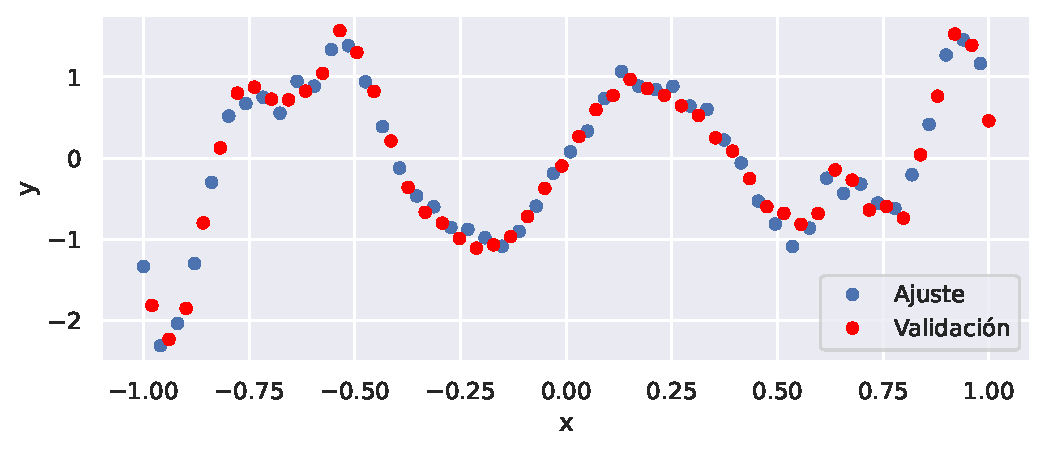
\includegraphics[width=0.85\textwidth]{img/scatterplot.pdf}
    \caption{
        Gráfico de dispersión del conjunto de datos. Se diferencian los datos pertenecientes a los conjuntos de ajuste y validación.
    } 
    \label{fig:scatterplot}
\end{figure}

El conjunto de datos que usamos está conformado por 100 observaciones de una variable $x$ y una variable $y$, particionados aleatoriamente en dos partes iguales, un conjunto de entrenamiento y un conjunto de validación (ver Figura \ref{fig:scatterplot}). A partir de estos datos, construimos la matriz $X$ según la expresión \ref{eq:matriz_x} con polinomios de Legendre de grado $d$.



Para hallar un modelo que generalice, buscamos el grado de polinomio $d$ y el valor de regularización $\lambda$ que minimizan el error de validación. En particular, tomamos como posibles valores $d={1, 2, \ldots, 49}$ y 100 valores $\lambda$ uniformemente distribuidos en una escala logarítimica en base 10 en el intervalo $[-7, 2]$, y evaluamos todas las combinaciones posibles (un total de $4900$ combinaciones). Para cada configuración, ajustamos el modelo con el algoritmo \ref{eq:cuadrados_svd_reg} en los datos de entrenamiento y evaluamos el ECM en los datos de validación según la expresión \ref{eq:ecm}.  

Realizamos todos los análisis y visualizaciones con Python 3.9. Para construir los polinomios de Legendre usamos la función \texttt{polynomial.legendre.legvander} de la biblioteca NumPy.



\section{Resultados} \label{sec:resultados}

En esta sección presentamos los resultados del análisis propuesto en la sección \ref{sec:experimentos}.

\begin{figure}[!ht]
    \centering
    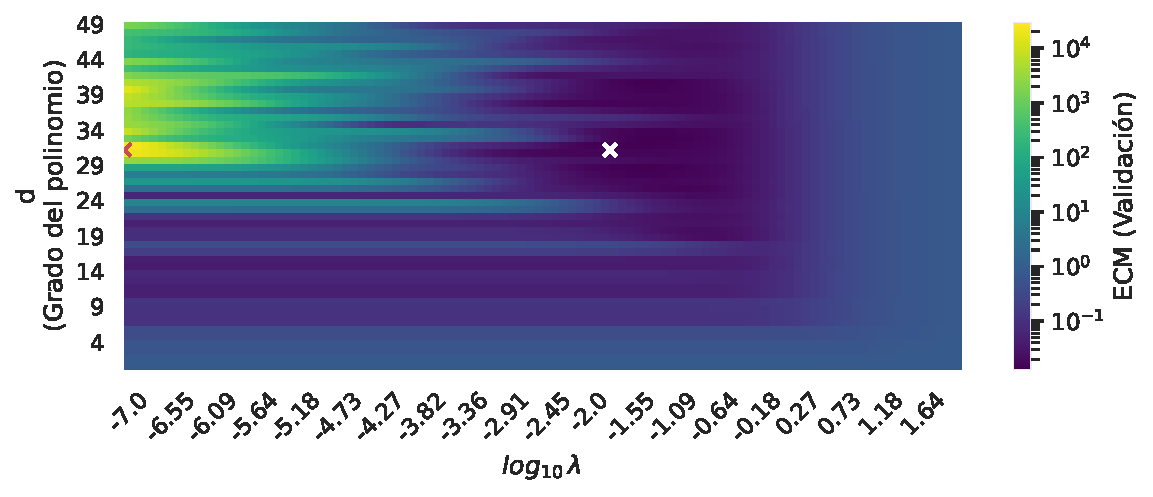
\includegraphics[width=0.85\textwidth]{img/heatmap.pdf}
    \caption{
        Mapa de calor que indica el error cuadrático medio de validación para la grilla de hiperparámetros explorada. En valores de $\lambda$ que exceden el rango visualizado, el error de validación no mejora. Se señala con una cruz blanca al punto asociado al par de ECM mínimo ($\lambda\approx 10^{-1.73}, d=32$), y con media cruz roja al asociado al de ECM máximo en todo el rango graficado ($\lambda=10^{-7}, d=32$).
    }
    \label{fig:heatmap}
\end{figure}

\clearpage
El ECM del ajuste a los datos de validación es mínimo para el polinomio de grado $d=32$ y coeficiente de regularización $\lambda \approx 10^{-1.73}$, con ECM $\approx 10^{-1.88}$. Casualmente, para el rango de hiperparámetros visualizado en el heatmap, $d=32$ es también el grado polinomial asociado al error máximo, con ECM $\approx 10^{4.47}$ (figura \ref{fig:heatmap}). El ajuste sobre los datos de validación mediante este polinomio puede ser visualizado en la figura \ref{fig:ajuste_mejor}.

\begin{figure}[!ht]
    \centering
    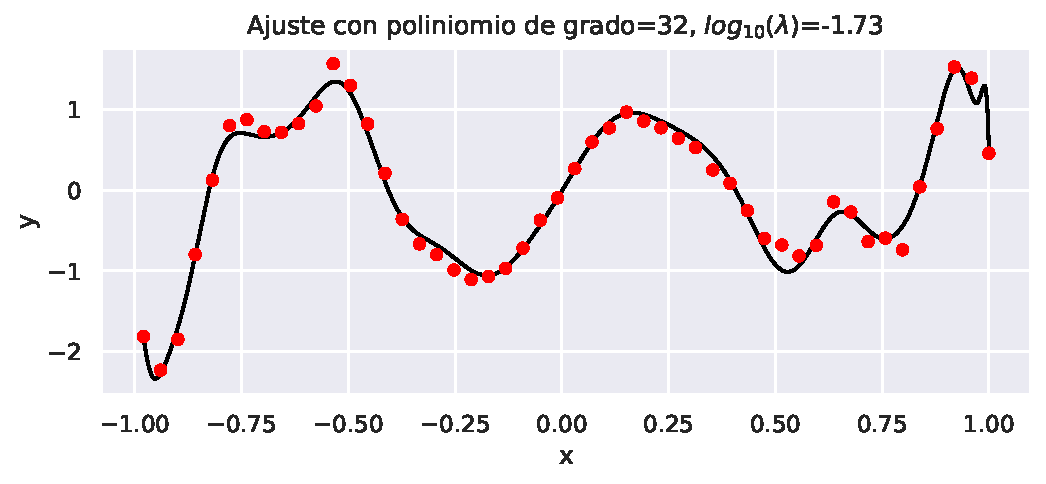
\includegraphics[width=0.85\textwidth]{img/ajuste_mejor.pdf}
    \caption{
        Valores ajustados del modelo con menor error de validación. En rojo, los datos de validación.
    } 
    \label{fig:ajuste_mejor}
\end{figure}

La figura \ref{fig:heatmap} expone varias propiedades interesantes del espacio de hiperparámetros ($\lambda$, $d$), que fueron exploradas en más profundidad en la figura \ref{fig:mas_ajustes} y que se comentan a continuación. 

Los máximos de ECM en todo el rango visualizado en el heatmap se encuentran en la región de alto grado polinomial y bajo coeficiente de regularización, donde es razonable que lo que esté ocurriendo sea un sobreajuste a los datos de entrenamiento y un consecuente mal ajuste en términos de ECM a los datos de validación. Esto puede visualizarse en la figura \ref{fig:ajuste_banda} para el caso particular con $d=32$, cuando se utilizan valores muy pequeños de $\lambda$. En relación a esto, una de las caracteristicas más llamativas del heatmap es la presencia de un bandeado horizontal para valores de $d$ suficientemente grandes ($d \gtrsim 20$), con la característica de que para $d$ fijo y al incrementar $\lambda$ el ECM tiende a primero disminuir hasta llegar a una región óptima para eventualmente volver a subir. Como puede visualizarse en la figura \ref{fig:ajuste_banda}, esto parece deberse a que con un primer incremento de $\lambda$ se logra disminuir el sobreajuste a los datos de entrenamiento; eventualmente se llega a un mínimo de ECM y el incremento de $\lambda$ más allá de este punto produce una disminución en la calidad del ajuste por exceso de regularización.

Para grados polinomiales muy bajos (alrededor de $d=3$) el ECM es, en terminos relativos a los errores en el resto del espacio, aproximadamente constante e independiente de $\lambda$ (moviendose horizontalmente a lo largo del heatmap con $d$ fijo). Esto evidentemente se debe a que cuando se tiene un grado polinomial demasiado bajo para los datos a ser ajustados, todo ajuste va a ser mediocre; no hay coeficiente de regularización que pueda salvar esa condición (figura \ref{fig:ajuste_grado_bajo}).

Finalmente, algo análogo ocurre para valores muy grandes de $\lambda$, más allá del valor óptimo hallado para $d=32$, para los cuales el ECM es aproximadamente constante e independiente del grado polinomial (moviendose verticalmente a lo largo del heatmap con $\lambda$ fijo). En este caso lo que ocurre es que para valores muy grandes de $\lambda$ el error de cuadrados mínimos pasa a ser dominado por el error de regularización, lo que produce que todos los coeficientes de la combinación lineal de polinomios de Legendre tiendan a 0, generandose como resultado un polinomio aproximadamente de la forma $f(x)=0$ independientemente del grado (figura \ref{fig:ajuste_exceso_ridge}).

\begin{figure}[htp]
\centering
    \subfloat[Polinomios de grado $d=32$ con coeficiente de regularización $\lambda$ variable. (*) Polinomio asociado al mejor ajuste (figuras \ref{fig:heatmap} y \ref{fig:ajuste_mejor}). En el gráfico de ECM en función de $\lambda$ se encuentra resaltado el punto asociado al polinomio. (**) Polinomio asociado al peor ajuste dentro del rango graficado en la figura \ref{fig:heatmap}.]{
    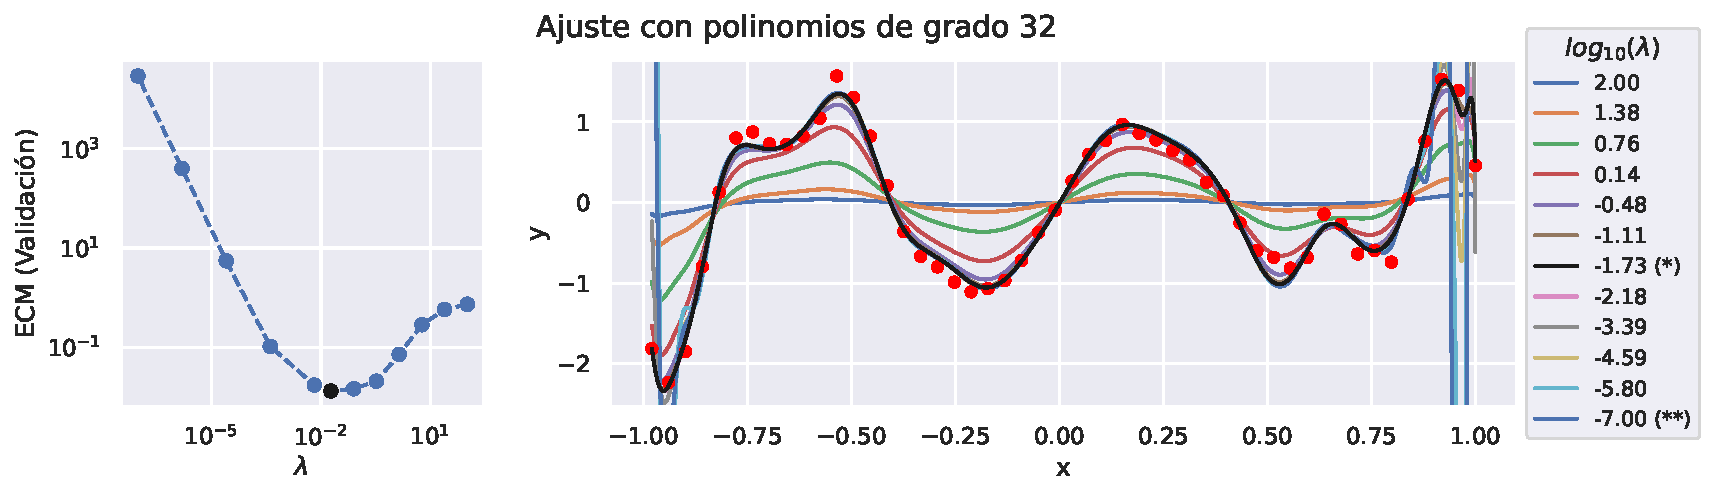
\includegraphics[width=1.0\textwidth]{img/ajuste_banda.pdf}
    \label{fig:ajuste_banda}
    }

    \subfloat[Polinomios de grado insuficiente $d=3$ con coeficiente de regularización $\lambda$ variable.]{
    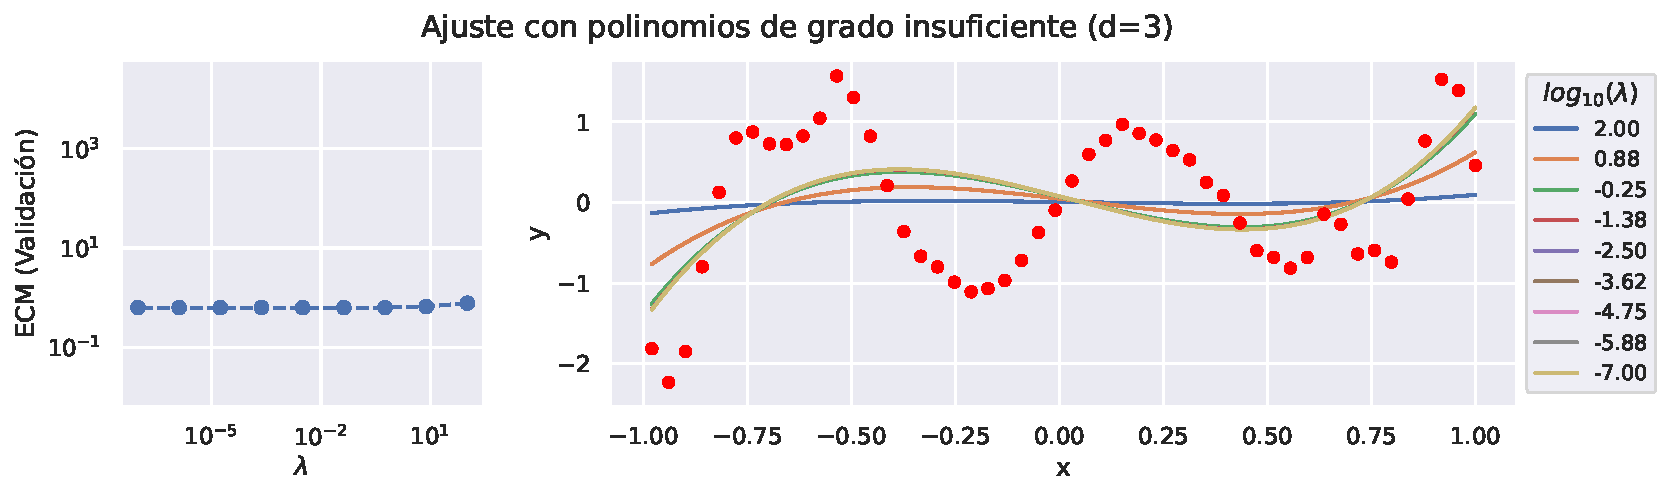
\includegraphics[width=1.00\textwidth]{img/ajuste_grado_bajo.pdf}
    \label{fig:ajuste_grado_bajo}
    }

    \subfloat[Polinomios de grado $d$ variable con coeficiente de regularización excesivo $\lambda=10$.]{
    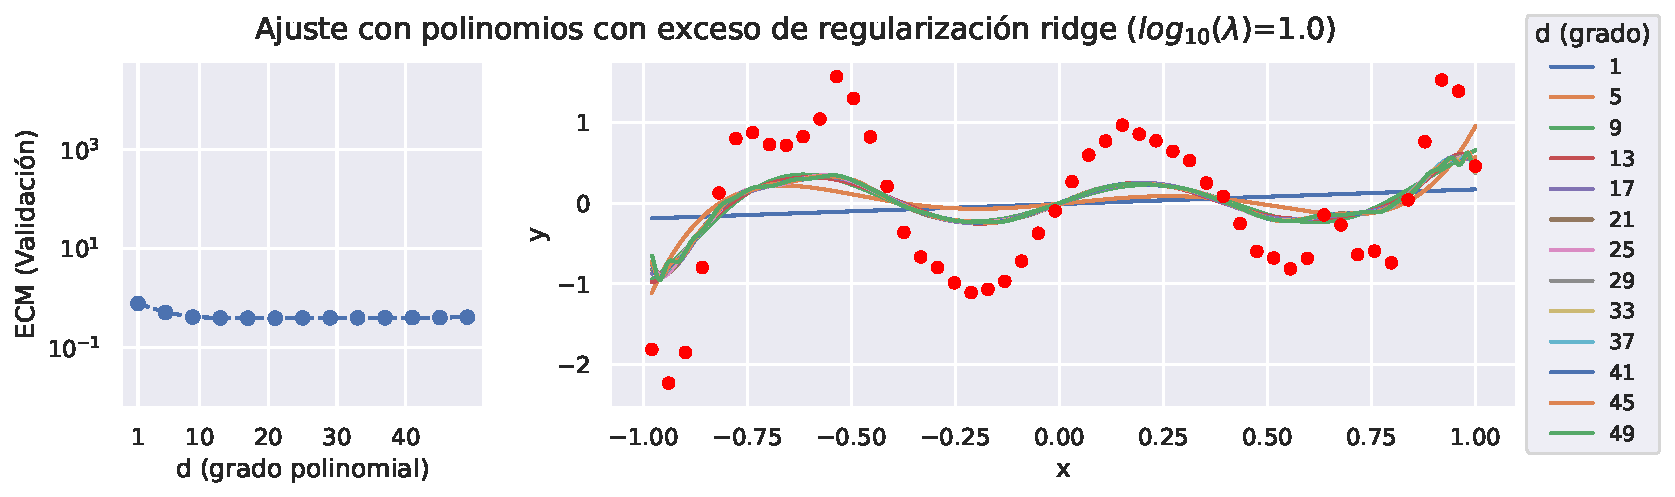
\includegraphics[width=1.0\textwidth]{img/ajuste_exceso_ridge.pdf}
    \label{fig:ajuste_exceso_ridge}
    }
    
    \caption{
        ECM y gráfico de ajuste a los datos de validación para polinomios asociados a series de pares ($\lambda, d$). En todos los casos se grafica a la izquierda el ECM de validación, en función de $\lambda$ en $(a)$ y $(b)$ y del grado polinomial en $(c)$, y a la derecha se muestran los ajustes correspondientes a cada valor del error, con los datos de validación en rojo. Para los gráficos de ECM se usó siempre la misma escala en el eje y con el fin facilitar la comparación de errores entre subfiguras.
    }
    \label{fig:mas_ajustes}
\end{figure}

\clearpage
\section{Conclusiones} \label{sec:conclusiones}

En este trabajo implementamos la solución al problema de mínimos cuadrados lineales mediante la descomposición SVD, con y sin regularización. También usamos la técnica de polinomios de Legendre para implementar regresión polinomial, la cual nos permite ajustar datos de manera no lineal resolviendo el problema de cuadrados mínimos lineales de manera computacionalmente eficiente. Mediante una aplicación práctica en la que buscamos el grado de polinomio y el valor de regularización que minimizan el error de validación, mostramos que la regularización es una estrategia efectiva para optimizar la capacidad predictiva de un modelo de ajuste.



%\section*{References}

%{
%\small

\bibliography{references}
\bibliographystyle{plainnat}

%}

%%%%%%%%%%%%%%%%%%%%%%%%%%%%%%%%%%%%%%%%%%%%%%%%%%%%%%%%%%%%

\end{document}